% Created 2020-08-20 Thu 15:50
% Intended LaTeX compiler: pdflatex
\documentclass[presentation]{beamer}
\usepackage[utf8]{inputenc}
\usepackage[T1]{fontenc}
\usepackage{graphicx}
\usepackage{grffile}
\usepackage{longtable}
\usepackage{wrapfig}
\usepackage{rotating}
\usepackage[normalem]{ulem}
\usepackage{amsmath}
\usepackage{textcomp}
\usepackage{amssymb}
\usepackage{capt-of}
\usepackage{hyperref}
\usepackage[margin=1cm]{geometry}
\usetheme{default}
\author{John Doe}
\date{\today}
\title{Functional Programming: Real World Performance, Nix and Warp Server}
\hypersetup{
 pdfauthor={John Doe},
 pdftitle={Functional Programming: Real World Performance, Nix and Warp Server},
 pdfkeywords={},
 pdfsubject={},
 pdfcreator={Emacs 26.3 (Org mode 9.4)}, 
 pdflang={English}}
\begin{document}

\maketitle
\begin{frame}{Outline}
\tableofcontents
\end{frame}

\begin{frame}[label={sec:org583bd86},fragile]{How Familiar is everyone with FP}
 \begin{block}{Disclaimer, not an expert}
\begin{itemize}
\item Logical fallacies will be used, not too fond of this but ¯$\backslash$\textsubscript{(ツ)}\_/¯.
\item Linux user for 7 years now
\begin{itemize}
\item Ubuntu
\item Proxmox
\item ArchLinux
\item Centos (server management)
\end{itemize}
\end{itemize}
\end{block}
\begin{block}{Choose some project}
\url{https://github.com/search?q=filename\%3Ashell.nix\&type=Code}
\end{block}
\begin{block}{Goals}
\begin{itemize}
\item Functional Programming \alert{Principles} (not only languages)
\item Academic mental exercise (hope not too boring):D
\begin{itemize}
\item not nessasarily useful
\item exposure to a \alert{what if?} world
\end{itemize}
\item No free lunch theorem
\begin{itemize}
\item PS: you get some free snacks with FP
\end{itemize}
\item confidence
\end{itemize}
\end{block}
\begin{block}{For whom is this talk for?}
\begin{itemize}
\item A rare case where FP's abilities can be shown
\item State management
\item DevOps
\item Images, Docker, VM, Clusters
\item give you a feel of \texttt{Nix}
\end{itemize}
\end{block}
\begin{block}{slant.co's opinions}
\begin{center}
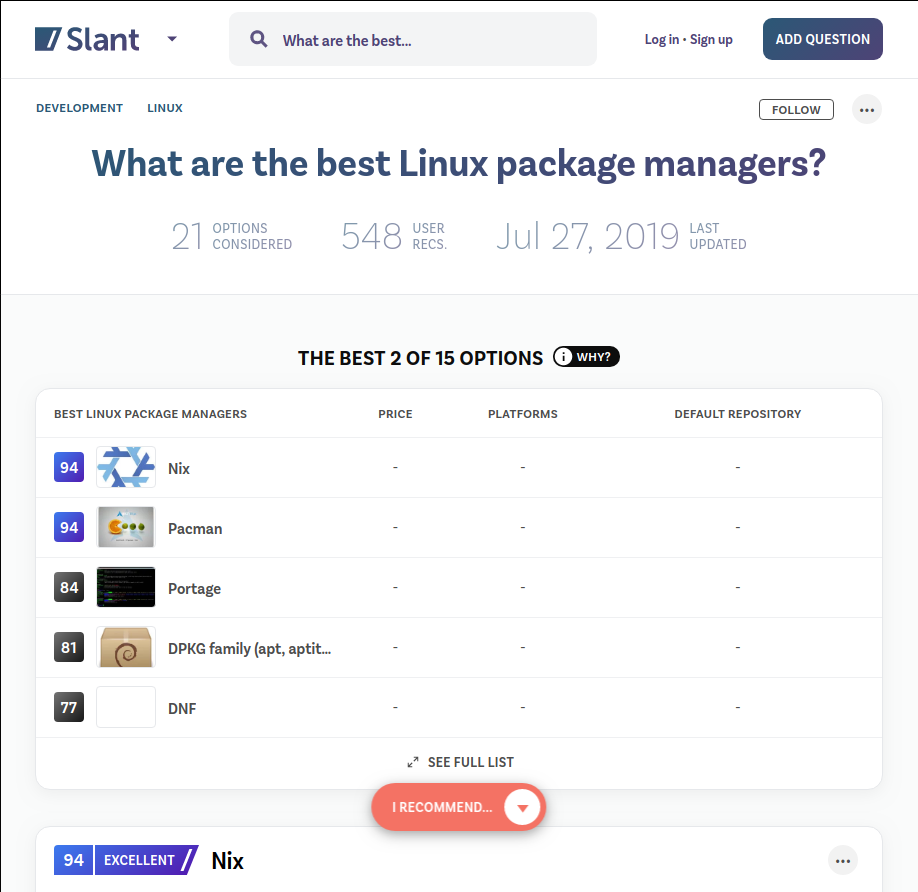
\includegraphics[width=.9\linewidth]{./images/screenshot-09.png}
\end{center}
\end{block}
\begin{block}{Really?}
\url{https://edolstra.github.io/pubs/nspfssd-lisa2004-final.pdf}
\url{https://edolstra.github.io/pubs/nixos-icfp2008-submitted.pdf}
\url{https://edolstra.github.io/pubs/phd-thesis.pdf}
\begin{center}

\includegraphics[width=.9\linewidth]{./images/screenshot-12.png}
\end{center}

\begin{center}

\includegraphics[width=.9\linewidth]{./images/screenshot-13.png}
\end{center}

\begin{center}

\includegraphics[width=.9\linewidth]{./images/screenshot-14.png}
\end{center}
\end{block}
\begin{block}{Functional Programming Primer}
\begin{itemize}
\item purity no side effects
\begin{itemize}
\item whats the point of a program if it cannot change any value?
\end{itemize}
\item everything is immutable
\begin{itemize}
\item \(x = 1; x = 2\)
\end{itemize}
\item lazy
\item memoize everything
\item extreme composability
\item keep as much information in the program as possible
\begin{itemize}
\item i.e. not a lot of reduce operations
\end{itemize}
\end{itemize}
\end{block}
\end{frame}
\begin{frame}[label={sec:org38cfab4},fragile]{What is the problem?}
 \begin{itemize}
\item Modern smart phones vs old phones
\item What OS has everyone used?
\begin{itemize}
\item windows
\item ubuntu/mac apt-get brew
\end{itemize}
\end{itemize}
\begin{block}{What is the problem?}
\begin{itemize}
\item multiple versions
\item mutability
\begin{itemize}
\item mysql-python
\end{itemize}
\item not accurate dependency graph
\item dependency hell
\end{itemize}
\end{block}
\begin{block}{Some modern day package management systems}
\begin{center}
\begin{tabular}{ll}
Package manager & Distributions\\
\hline
apt, apt-get & Debian, Ubuntu\\
rpm, yum & Redhat, Centos\\
pacman & ArchLinux\\
brew & MacOS\\
\end{tabular}
\end{center}
\end{block}
\begin{block}{What about sub ecosystems?}
\begin{center}
\begin{tabular}{ll}
Package manager & ???\\
\hline
pip, virtualenv, pipenv & Python2,3(???)\\
npm, yarn & Nodejs\\
cabal, stack, hackage & Haskell :)\\
go? & go?\\
brew & MacOS\\
use-package, vim, fish, zsh & \ldots{}\\
\end{tabular}
\end{center}
\end{block}
\begin{block}{How to make a package manager?}
\begin{itemize}
\item What are the basic parts that we need?
\end{itemize}
\end{block}
\begin{block}{How to make a package manager?}
\begin{center}
\begin{tabular}{ll}
build dependencies & What do I need to build the program?\\
runtime dependencies & What \texttt{.so} shared objects do I need?\\
configurations & What in \texttt{/etc/...} config files\\
\end{tabular}
\end{center}
\begin{itemize}
\item essentially think of it as a graph, whenever we upgrade or install a package,
we are mutating a node on this graph to point to something else.
\end{itemize}
\begin{block}{real senario}
\begin{verbatim}
  pkgname=pacman
  pkgver=5.1.0
  _pkgver=1.0.0
  pkgrel=2
  pkgdesc="A library-based package manager with dependency support"
  arch=('i686' 'x86_64')
  url="http://www.archlinux.org/pacman/"
  license=('GPL')
  groups=('base' 'base-devel')
  depends=('bash>=4.2.042-2' 'glibc>=2.17-2' 'libarchive>=3.1.2' 'curl>=7.39.0'
           'gpgme' 'archlinux-keyring' 'manjaro-keyring' 'pacman-mirrors>=4.1.0')
  checkdepends=('python2' 'fakechroot')
  makedepends=('asciidoc' 'pacman>=5.1')
  optdepends=('haveged: for pacman-init.service')
  provides=('pacman-contrib' 'pacman-init')
  conflicts=('pacman-contrib' 'pacman-init')
  replaces=('pacman-contrib' 'pacman-init')
  backup=(etc/pacman.conf etc/makepkg.conf)
  install=pacman.install
  options=('strip' 'debug')
\end{verbatim}
\end{block}
\end{block}
\begin{block}{Problems with modern package management}
\url{https://wiki.debian.org/DontBreakDebian\#Don.27t\_make\_a\_FrankenDebian}
\begin{center}
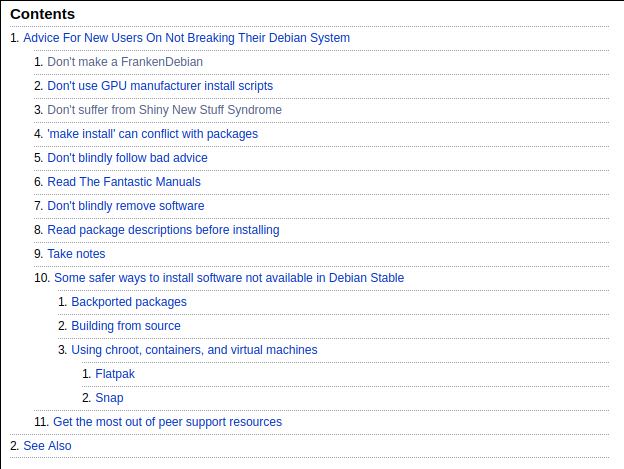
\includegraphics[width=.9\linewidth]{./images/screenshot-01.png}
\end{center}
\end{block}
\begin{block}{Why imperative is bad? What is so imperative about installing packages?}
Mutation
\end{block}
\begin{block}{Are you familiar with \texttt{DEPENDENCY HELL}?}
\begin{itemize}
\item \url{https://www.reddit.com/r/ProgrammerHumor/comments/75txp4/nodejs\_dependency\_hell\_visualized\_for\_the\_first/?utm\_source=share\&utm\_medium=web2x}
\item \url{https://github.com/vector-im/riot-web/network/dependencies}
\end{itemize}
\end{block}
\begin{block}{All types of ``DEPENDENCY HELL''}
\url{https://miro.medium.com/max/984/0*7ezJOtYUkI5zyqWU.png}
\begin{itemize}
\item \{ DLL, dependency, npm, cabal \} hell, different names for the same demon
\item conflicting dependency
\begin{itemize}
\item shared components like library links \texttt{cuda.7.so} vs \texttt{cuda.6.so}
\end{itemize}
\item multiple version side by side and roll backs
\item possible solutions
\begin{itemize}
\item set of stable packages like \texttt{Debian} or \texttt{haskell stack snapshots}
\end{itemize}
\end{itemize}
\end{block}
\begin{block}{Not Atomic 01}
\begin{itemize}
\item kill upgrades half way
\begin{itemize}
\item packages left in a semi updated state
\item sometimes need to manually remove lock files
\end{itemize}
\end{itemize}
\begin{verbatim}
   COMMAND   PID USER   FD   TYPE DEVICE SIZE/OFF   NODE NAME
   dpkg    29329 root    3uW  REG    8,7        0 262367 /var/lib/dpkg/lock
\end{verbatim}
\end{block}
\begin{block}{Not Atomic 02}
\begin{itemize}
\item can be fixed but kinda troublesome.
\end{itemize}
\begin{center}
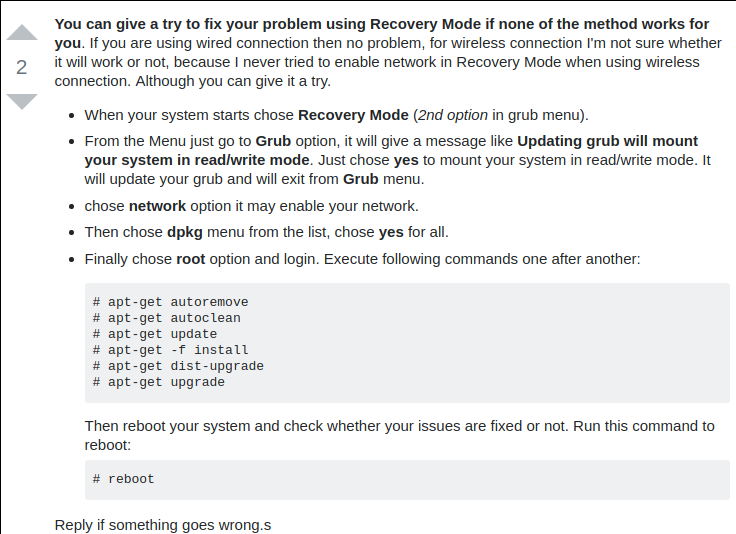
\includegraphics[width=.9\linewidth]{./images/screenshot-02.png}
\end{center}
\end{block}
\begin{block}{Whats bad about imperative summary?}
\begin{itemize}
\item No Variability
\begin{itemize}
\item cannot point to older versions of the same thing
\end{itemize}
\item Dependency hell
\begin{itemize}
\item conflicting dependencies
\end{itemize}
\item Not atomic upgrades
\begin{itemize}
\item unknown state if break half way
\end{itemize}
\end{itemize}
These problems are really similar to the problems with imperative languages!
like \texttt{JAVA} and people have already made solutions for them like how \texttt{Haskell}
does. We could learn a thing or two from them.
\end{block}
\end{frame}
\begin{frame}[label={sec:org72632d2},fragile]{What it should/could/would have been?}
 \begin{itemize}
\item Imagine now that we implemented all the things of a functional programming
language to create a functional package management system?
\item What can we do with this?
\end{itemize}
\begin{block}{GUIX vs Nix}
\begin{itemize}
\item \begin{center}

\includegraphics[width=.9\linewidth]{./images/screenshot-04.png}
\end{center}
\item \begin{center}
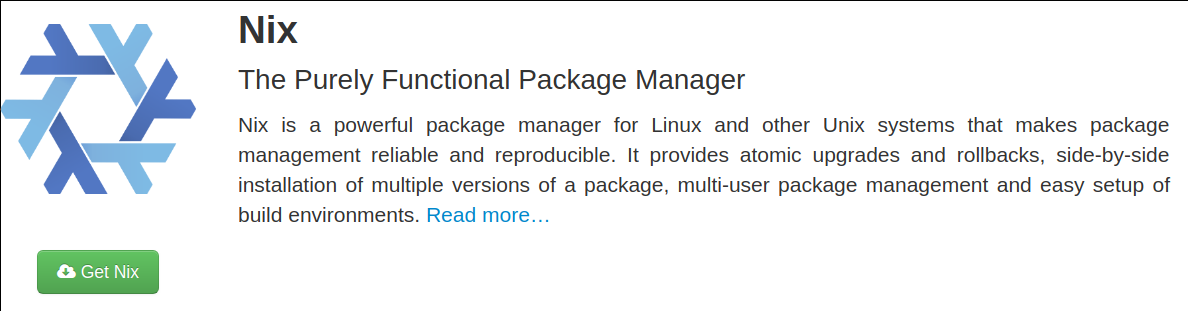
\includegraphics[width=.9\linewidth]{./images/screenshot-03.png}
\end{center}
\end{itemize}
\end{block}
\begin{block}{Introducing Nix Package Management}
\begin{itemize}
\item solves all of the problems above
\begin{itemize}
\item Can point to different versions of the same thing
\begin{itemize}
\item cannot point to older versions of the same thing
\end{itemize}
\item Dependency hell
\item Not atomic upgrades
\begin{itemize}
\item unknown state if break half way
\end{itemize}
\end{itemize}
\end{itemize}
\end{block}
\begin{block}{Main mechanism}
\begin{itemize}
\item install everything in path \texttt{/nix/store/\{hash\}-name}
\item via \texttt{symlinking}
\end{itemize}
\end{block}
\begin{block}{What you get for free with this mechanism?}
\begin{itemize}
\item no \texttt{sudo}
\item easy revert and roll back
\item select specific version
\item 2 different version can run at the same time
\item same \alert{development} environment as the \alert{runtime} environment!
\begin{itemize}
\item nix-shell
\end{itemize}
\end{itemize}
\begin{block}{no \texttt{sudo}, where is my \texttt{sudo}?}
\begin{itemize}
\item linux was developed as a \texttt{time sharing} system
\item many users were expected to share a single computer.
\item thus to manage conflicts, a \texttt{super user}, \texttt{root} was required to
install and manage packages
\end{itemize}
\begin{verbatim}
nix-env -iA nixos.figlet
\end{verbatim}
\end{block}

\begin{block}{easy revert, rollback}
\begin{verbatim}
      figlet "I am here!"
\end{verbatim}
\begin{verbatim}
      nix-env --rollback
\end{verbatim}
\begin{verbatim}
      figlet "are you still here?"
\end{verbatim}
\end{block}
\begin{block}{Select specific version}
\begin{verbatim}
      cd ~/projects/nix-config/
      git checkout ??
      nix-env -f ~/projects/nix-config/ -iA screenfetch
\end{verbatim}
screenfetch 2016 vs current
\end{block}
\begin{block}{Installing and running 2 version of same software}
\begin{verbatim}
      stack --version
      su
      stack --version
\end{verbatim}
\end{block}
\begin{block}{Same development environment and runtime environment}
\begin{itemize}
\item I am not an electrical engineer or something but I program my
own keyboard. So I need some sort of firmware flasher. like
\texttt{dfuprogrammer} I dont need it on my system.
\end{itemize}
\begin{verbatim}
      cd ~/projects/qmk_firmware/
      make
      dfuprogrammer
      nix-shell
      make
      dfuprogrammer
\end{verbatim}
\end{block}
\end{block}
\begin{block}{Going all the way, NixOS}
\begin{itemize}
\item whole system management via Nix and thus NixOS
\begin{itemize}
\item Version controlled operating system
\item show OS reboot
\item I wanted to show my generations so had been delaying removing
my older generations
\end{itemize}
\end{itemize}
\begin{verbatim}
     df -h /
     nix-collect-garbage --delete-older-than 10 --dry-run
\end{verbatim}
\begin{block}{NixOS}
\begin{itemize}
\item show \url{file:///home/df/nix-config/configuration.nix}
\item python package management \url{file:///home/df/nix-config/configuration.nix}
\item gnupg agent \url{file:///home/df/nix-config/configuration.nix}
\item ports \url{file:///home/df/nix-config/configuration.nix}
\begin{itemize}
\item I think it helps me get a state of all the ports in one place
\end{itemize}
\item users and security all in one place
\url{file:///home/df/nix-config/configuration.nix}
\begin{itemize}
\item authorisedkeys
\end{itemize}
\item postgresql can be packaged in \texttt{shell.nix}
\url{file:///home/df/nix-config/configuration.nix}
\begin{itemize}
\item separate project called \texttt{nixos-shell}
\url{https://github.com/chrisfarms/nixos-shell}
\end{itemize}
\item filesystems \url{file:///etc/nixos/hardware-configuration.nix}
\end{itemize}
\end{block}
\begin{block}{docker}
\url{https://nixos.wiki/wiki/Docker}
\begin{verbatim}
      virtualisation.docker.enable = true;
      users.users.<myuser>.extraGroups = [ "docker" ];
\end{verbatim}
\begin{verbatim}
      nix-build '<nixpkgs>' -A dockerTools.examples.redis
      docker load < result
\end{verbatim}
\url{https://github.com/NixOS/nixpkgs/blob/master/pkgs/build-support/docker/examples.nix}
\end{block}
\begin{block}{easy cd/dvd}
\begin{verbatim}
      cd ~/projects/nixpkgs
      nix-build -A config.system.build.isoImage -I nixos-config=modules/installer/cd-dvd/installation-cd-minimal.nix default.nix
\end{verbatim}
\end{block}
\begin{block}{easy vm}
\begin{verbatim}
      cd ./nixops
      nixops create -d simple02 network.nix
      nixops deploy -d simple02
\end{verbatim}
\begin{verbatim}
      deployment.targetEnv = "ec2";
      deployment.region = "eu-west-1";
\end{verbatim}
\end{block}
\end{block}
\end{frame}
\begin{frame}[label={sec:org6d29320},fragile]{How does nix actually work?}
 \begin{block}{Nix expressions}
\begin{itemize}
\item functional expressions, not general purpose please do not program
things with it
\item comes with its own BNF grammar
\end{itemize}
\begin{center}
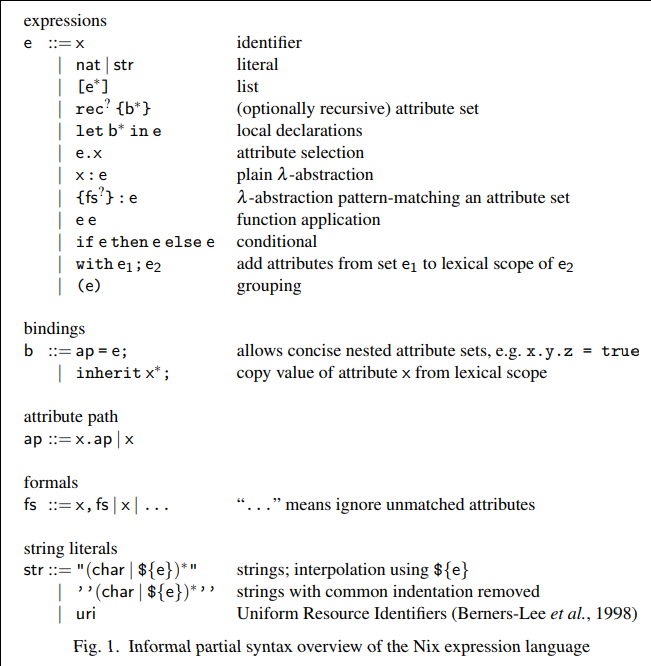
\includegraphics[width=.9\linewidth]{./images/screenshot-05.png}
\end{center}
\end{block}
\begin{block}{Language features}
\begin{itemize}
\item Nix expressions
\begin{itemize}
\item dynamically typed
\item lazy
\item pure
\end{itemize}
\end{itemize}
\end{block}
\begin{block}{The main point}
\begin{itemize}
\item Nix expressions are here to describe a graph of build actions
called \texttt{derivations}
\begin{itemize}
\item build script
\item set of environment variables
\item set of dependencies
\end{itemize}
\end{itemize}
\end{block}
\begin{block}{Example: Xmonad}
\begin{center}
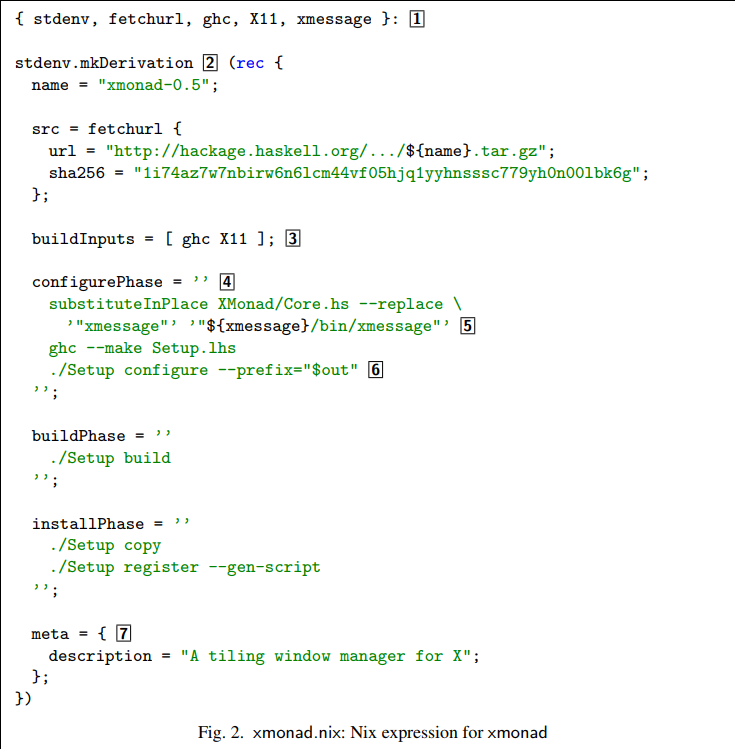
\includegraphics[width=.9\linewidth]{./images/screenshot-06.png}
\end{center}
\end{block}
\begin{block}{Example: Xmonad}
\begin{center}
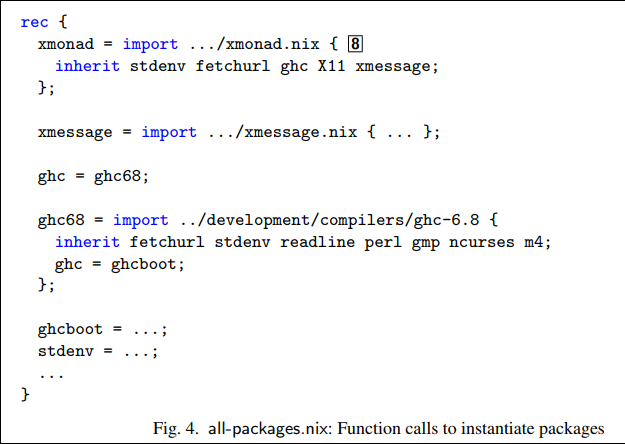
\includegraphics[width=.9\linewidth]{./images/screenshot-07.png}
\end{center}
\end{block}
\begin{block}{Main mechanism}
\begin{center}
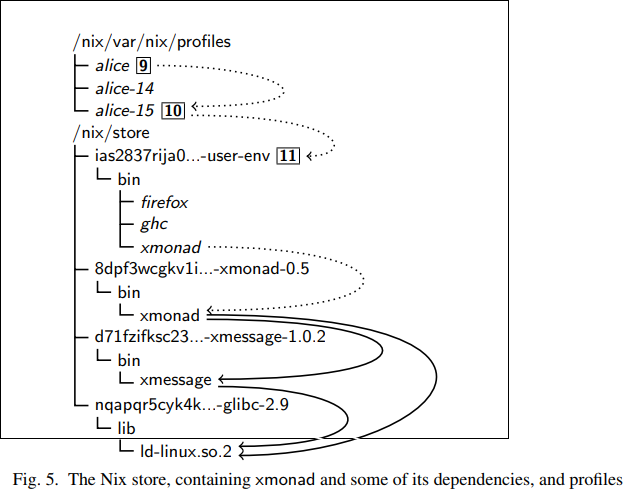
\includegraphics[width=.9\linewidth]{./images/screenshot-08.png}
\end{center}
\end{block}
\end{frame}
\begin{frame}[label={sec:orgf2c370a},fragile]{Nix as infrastructure (imagination)}
 \begin{itemize}
\item how might one use nix in \texttt{JPMC's} infrastructure?
\end{itemize}
\begin{block}{Main componenets}
\begin{itemize}
\item Hydra caching
\item Dependency management
\item Ease of use
\begin{itemize}
\item nix-shell
\end{itemize}
\item Security
\end{itemize}
\end{block}
\begin{block}{Caching build farm or cachix}
\begin{center}
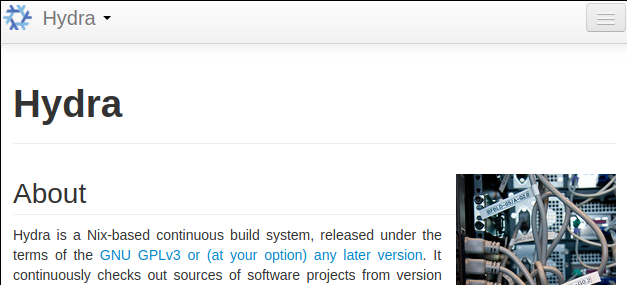
\includegraphics[width=.9\linewidth]{./images/screenshot-10.png}
\end{center}
\begin{center}

\includegraphics[width=.9\linewidth]{./images/screenshot-11.png}
\end{center}
\end{block}
\end{frame}
\begin{frame}[label={sec:orgd1c54e1}]{references}
\begin{itemize}
\item\relax [HTML] Nix: A Safe and Policy-Free System for Software Deployment.
\begin{itemize}
\item E Dolstra, M De Jonge, E Visser - usenix.org
\item \url{https://nixos.org/\~eelco/pubs/nspfssd-lisa2004-final.pdf}
\end{itemize}
\item\relax [PDF] A Purely Functional Linux Distribution - NixOS
\begin{itemize}
\item E Dolstra
\item \url{https://nixos.org/\~eelco/pubs/nixos-jfp-final.pdf}
\end{itemize}
\item Hydra - NixOS
\begin{itemize}
\item \url{https://nixos.org/\~eelco/pubs/hydra-scp-submitted.pdf}
\end{itemize}
\end{itemize}
\end{frame}
\begin{frame}[label={sec:org785492e},fragile]{Part 2 Warp optimization}
 \begin{center}

\includegraphics[width=.9\linewidth]{Part_2_Warp_optimization/2020-08-20_14-51-11_screenshot.png}
\end{center}

\url{https://www.aosabook.org/en/posa/warp.html}
\begin{block}{2013 Results}
\begin{center}
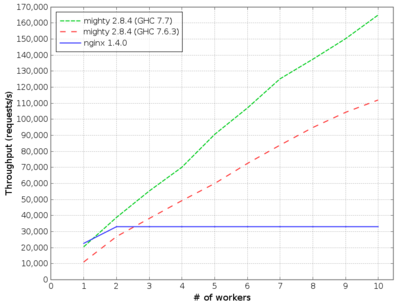
\includegraphics[width=.9\linewidth]{Part_2_warp/2020-08-20_14-50-23_screenshot.png}
\end{center}
\end{block}
\begin{block}{Overall Architecture}
\begin{center}
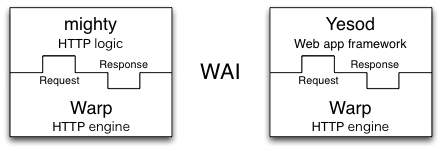
\includegraphics[width=.9\linewidth]{Part_2_Warp_optimization/2020-08-20_15-46-34_screenshot.png}
\end{center}
\end{block}
\begin{block}{Type and life cycle}
\begin{verbatim}
type Application = Request -> ResourceT IO Response
\end{verbatim}

\begin{center}
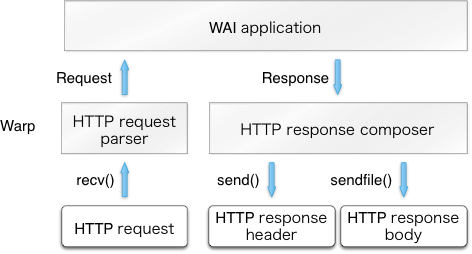
\includegraphics[width=.9\linewidth]{Part_2_Warp_optimization/2020-08-20_15-47-23_screenshot.png}
\end{center}
\end{block}
\begin{block}{Threads}
user threads
\end{block}
\begin{block}{As little syscalls as possible}
\begin{itemize}
\item use strace to check what nginx was doing
\item found \texttt{accept4}
\end{itemize}
\end{block}
\begin{block}{Profiling}
\begin{itemize}
\item the date string format is taking up most of the cpu time
\item so they made a cache for that
\item btw haskell by default memoised every thing
\end{itemize}
\end{block}
\begin{block}{Avoiding locks}
they used compare and swap instead
\end{block}

\begin{block}{Using proper datastructure}
\begin{itemize}
\item \texttt{String} in haskell is actually a \texttt{List} of \texttt{Char}
\begin{itemize}
\item \texttt{List} as in \texttt{Linked-lists}
\end{itemize}
\item \texttt{ByteString} so you can do \texttt{splicing} like \texttt{GO}.
\begin{itemize}
\item implemented in low level \texttt{C}
\end{itemize}
\item Handroll several components to avoid overhead like the parsing library
\end{itemize}
\end{block}
\begin{block}{ByteString splicing}
Everything in haskell by default is immutable so multiple threads can read it at the same time with no issues.

Updates are done with compare and swap.
\begin{center}
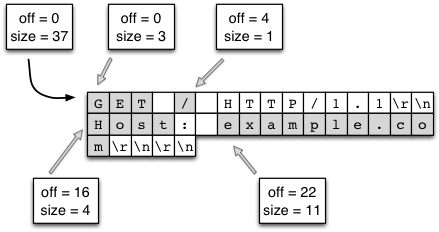
\includegraphics[width=.9\linewidth]{ByteString_splicing/2020-08-20_15-39-39_screenshot.png}
\end{center}
\end{block}
\end{frame}
\end{document}
